\documentclass[a4paper, 11pt]{article}

%%--LANGUAGE AND ENCODING--%%
\usepackage[swedish]{babel}
\usepackage[english,cleanlook]{isodate}%
\usepackage[utf8]{inputenc}
\usepackage{csquotes}

\usepackage[yyyymmdd]{datetime}
\renewcommand{\dateseparator}{--}

\usepackage{xfrac}

%%--BIBLOPGRAPHY--%%
\usepackage[backend=biber, natbib=true, urldate=iso8601, maxnames=2, minnames=1, maxbibnames=10, minbibnames=6, citestyle=numeric-comp, sorting=none, firstinits=true]{biblatex}

%%--SPACING AND MARGIN--%
\usepackage[textwidth=140mm]{geometry}
%\usepackage[margin=3.5cm, top=2.5cm]{geometry}
\setlength{\parindent}{0mm}


%%--SANS-SERIF FONTS FOR SECTIONS--%%
\usepackage{sectsty}
\usepackage{helvet}
\allsectionsfont{\bfseries\sffamily}

%%Links within the doc%%
\usepackage[hidelinks]{hyperref}
%%--GRAPHICS--%%  (Requires preamble)
% \usepackage{tikz}
\usepackage{graphicx}
\usepackage{caption}
\usepackage[justification=centering]{caption}
\usepackage{subcaption}


%%--ADVANCE TABULARS--%%
\usepackage{tabularx}
\def\arraystretch{1.3}
%PREAMBLE%
%%-SECTION NUMMBERING DEPTH-%%
%\setcounter{secnumdepth}{3} %3=Default

\hyphenation{pa-nel-en instruktion-er sol-panel-en fatt-ades anse nu-varande av-sedda fungera-nde  kommunikations-stand-ard-er version-er mot-svarande enkorts-dator enhet-ens exempel-vis operativ-system doku-ment-ation platt-forms-oberoende system-utvecklings-metoden} 

%%-GRAPHICS-%%
\DeclareGraphicsExtensions{.pdf,.png,.jpg}

%%-BIBLIOGRAPHY-%%
%Adds references library and formats it.
% To  refere to a reference in the library use  \cite{} for ieee
\addbibresource{ref.bib} \setlength{\bibitemsep}{\baselineskip} 
%Always shows the authors in bibliography as Lastname, Firstname
%\DeclareNameAlias{sortname}{last-first} 

%%-DOCUMENT INFORMATION-%%
%Header/Footer%
\author{Svedberg, Pär\\ \texttt{svpar@student.chalmers.se}  \\ 
            19821112--7652 \and
            Åkergren, Oskar\\ \texttt{akergren@student.chalmers.se}  \\ 19880508--7114
}
\title{\underline{UTKAST} \\ Kalibrering av ljussensor \\ för Parans solpanel \vspace{1cm}}

\date{\vspace{8cm}\today}

\begin{document}
\maketitle
\begin{center}
    Version 0.11    
\end{center}

\thispagestyle{empty}

\newpage
\setcounter{page}{1}
\pagenumbering{roman}

\renewcommand{\abstractname}{Abstract}
\begin{abstract}
    \noindent The aim of this project is to automatically calibrate a photo sensor on a sun panel that is following the sun in its path, to maximize the light intake that is to be used as a light source in doors, a calibration that was originally made by hand. The project was performed in iterations according to a design science research method and has two main focus tasks. The first is to develop a calibration algorithm and the second is suggest a communication solution between the room and the panel. The result of the project is a fully functioning calibration application, and two suggestions for the communication where the fibre optic cables is used to transport the data. \medskip

    \noindent \textbf{Keywords:} Calibration, RS-232, serial communication, optical commication, fibreoptics, microcontroller, indoor lighting, Parans, light sensor
\end{abstract}

\renewcommand{\abstractname}{Sammandrag}
\begin{abstract}
    \noindent Detta projekt syftar till att möjliggöra en automatisk kalibrering av fotosensorn på en solpanel som aktivt följer solen för att maximera dess solintag som nyttjas till belysning, en kalibrering som tidigare utförts manuellt. Projektet har genomförts i iterationer med stöd av en 'design science research'-metod och är fokuserat på två huvudsakliga områden, dels en effektiv kalibreringsalgoritm och dels en kommunikationslösning mellan solpanelen och det rum som panelen lyser upp. Projektet har resulterat i en färdig mjukvarulösning som kalibrerar panelen och projektet har lämnat två förslag på lösningar gällande kommunikationen, där vi rekommenderar att använda panelens egna fiberkablar som datamedium. \medskip

    \noindent \textbf{Nyckelord:} Kalibrering, RS-232, seriell kommunikation, optisk kommunikation, fiberoptik, mikrokonroller, belysning, Parans, ljussensor
\end{abstract}

\newpage
\subsection*{Förord} % (fold)
\label{sub:f_rord}
    Detta examensarbete skrivs inom ramen för kursen LMTX38, Examensarbete vid Data- och informationsteknik vårterminen 2015 på Chalmers tekniska högskola. \bigskip

    Författarna vill rikta ett stort tack till Parans Solar Lighting AB för tillhandahållande av materiel som projektet nyttjat sig av, lokal att arbeta i och stöd vid arbetet. Ett särskilt tack riktas till handledare Karl Nilsson vid Parans för förslaget till examensarbetets problemområde och avsatt tid för handledning av projektet. Vi riktar även ett tack till Simon Larsson vid Parans för bollande av idéer och stöttande vid utvecklingsarbetet. Vidare vill vi tacka handledare Lennart Hansson vid Chalmers för hans stöd vid skrivande av denna rapport och förslag för att driva arbetet framåt. Ett avslutande tack skickas till Sakib Sistek vid Chalmers för hans förmedling av kontakten till Parans och hans hjälp vid förberedningen till detta examensarbete.

% subsection f_rord (end)

\newpage

\subsection*{Beteckningar} % (fold)
\label{sub:beteckningar}
    \begin{tabularx}{\textwidth}{@{}rX}
        C & Programmeringsspråk \\
        I/O & Input/Output \\
        I²C & Standard för synkron seriell datakommunikation \\
        lm & lumen, SI-enhet för ljusflöde \\
        lux & SI-enhet för belysning, 1 lux = 1 $\sfrac{\text{lm}}{\text{m}^2}$ \\
        RS-232 & Standard för asynkron seriell datakommunikation \\
        UART & Universal Asynchronous Receiver/Transmitter, gränssnitt för seriell kommunikation
        
    \end{tabularx}
% subsection beteckningar (end)

\newpage
\tableofcontents
\listoffigures
\listoftables

\newpage

\setcounter{page}{1}
\pagenumbering{arabic}

\section{Introduktion} % (fold)
\label{sec:indroduktion}

    \subsection{Bakgrund} % (fold)
    \label{sub:bakgrund}
        Parans är utvecklare av en produkt som via optiska fibrer levererar naturligt solljus in i byggnader som ett alternativ till dagens traditionella ljuskällor. 
        Bolaget är baserat i Göteborg men levererar systemen globalt och har flera installationer runt om i världen. \bigskip

        Produkten fokuserar in solljus i optiska fibrer och styrs med hjälp av två stegmotorer för att följa solens bana. 
        Styrningen sker med en algoritm som ger solposition i grader, baserat på installationsplatsens geografiska position och tid, och för finare styrning av panelen då solen är framme inhämtas data från en ljussensor med fotocell.
        Detta för att alltid maximera det solljus som fokuseras in i fibern.\bigskip

        Styrkortet och motorerna till panelen drivs av en spänning om tolv (12) volt och kortet är en egen design kring mikrokontrollen PIC32. 
        Källkoden till panelen är skriven i \texttt{C} och kommunikation till enheten sker via seriell förbindelse över USB, där en USB till RS-232-omvandlare är integrerad på styrkortet. För att skicka instruktioner till panelen används en terminalemulator. \bigskip

        Ljussensorn som används i solpanelen kan representeras som ett koordinatsystem där sensorn som standard förväntar sig att ljuset fokuseras till en punkt som träffar origo. 
        Problemet som Parans har är tudelat. Det första problemet är att linsen vid tillverkning av panelen kan fokusera ljuset något vid sidan av origo på sensorn, vilket leder till sämre ljusintag till de optiska fibrerna. 
        Det andra problemet är att solen inte går att fokusera ned till en punkt, utan kommer alltid att representeras som en disk, vilket kan leda till en mätosäkerhet hos sensorn och då även sämre ljusintag till de optiska fibrerna. \bigskip

        Sensorn kalibreras genom att flytta punkten på det koordinatsystem som ljuset fokuseras ned till. Idag använder Parans en manuell metod där en terminalemulator används för att ange kommandon som vrider solpanelen och sedan kontrolleras värdet på en separat luxmätare.
    % subsection bakgrund (end)

    \subsection{Syfte} % (fold)
    \label{sub:syfte}
          Syftet med projektet är att möjliggöra en helt automatisk process som kan kalibrera fotosensorn i Parans solpaneler så att maximalt ljusflöde från panelen kan uppnås. Syftet med processen är att minska tidsåtgången och höja precisionen jämfört med dagens manuella metod. 
          Vidare syftar projektet till att möjliggöra kommunikation mellan panelen och en luxmätare inne i byggnaden, så att kalibreringstekniken kan nyttjas till systemen generellt, oavsett om de är tagna i bruk eller i fabrik.
    % subsection syfte (end)

    \subsection{Mål} % (fold)
    \label{sub:mal}
        Målet med det här projektet är att ta fram en produkt som justerar fokuspunkten på ljussensorn, vilket då vrider på solpanelen för att lokalisera de x- och y-värden där intaget av solljus är som störst. 
        Ljusstyrkan mäts med hjälp av en luxmätare som levererar ljusintaget till en dator eller till en annan programmerbar enhet. 
        När det maximala ljusintaget är uppmätt registreras x- och y-värdena som den nya fokuspunkten för ljussensorn istället för det förinställda värdet på origo. 
        Vidare är målet med produkten att den ska stödja kommunikation mellan en luxmätare inne i byggnaden och en panel som befinner sig på taket. 
    % section mal (end)


    \subsection{Frågeställning} % (fold)
    \label{sub:fragestallning}
        \begin{itemize}
            \item Vilken algoritm kan anses vara lämplig för kalibreringen?
            \item Vilka förutsättningar för kommunikation finns mellan solpanelen och det upplysta rummet? 
            \item Hur tillförlitligt är det valda kommunikationssättet? 
            
        \end{itemize}
    % subsection fr_gest_llning (end)

    \subsection{Avgränsningar} % (fold)
    \label{sub:avgr_nsningar}
        \subsubsection{Hårdvara} % (fold)
        \label{ssub:h_rdvara}
            Redan existerande hårdvara kommer att användas, det vill säga sådan avsedd att användas för de ändamål nödvändiga för projektet. 
            Den primära hårdvaran, solpanel och luxmätare, kommer att tillhandahållas av uppdragsgivaren och inga alternativ till dessa kommer att undersökas. 
            Eventuell övrig hårdvara kan antingen vara helhetslösningar eller sådana som löser delproblem och kombineras. 
            De lösningar som kommer att undersökas och utvecklas är begränsade till att stödja företagets panel SP3.
        % subsection h_rdvara (end)

        \subsubsection{Mjukvara} % (fold)
        \label{ssub:mjukvara}
            Mjukvara kommer att utvecklas för att nå projektets uppsatta mål. 
            Denna kan komma att inkludera användning av både medföljande och externa ramverk och bibliotek för att lösa olika delproblem, exempelvis grafisk framställning och kommunikation mellan olika enheter.
        % subsection mjukvara (end)

    % section avgr_nsningar (end)

% section indroduktion (end)
\section{Metod} % (fold)
\label{sec:metod}
    
    \subsection{Vetenskaplig metod} % (fold)
    \label{sub:vetenskaplig_metod}
    	Detta projekt har tillämpat en variant av den vetenskapliga metoden Design Science Research (DSR). Metoden anses lämplig till problemlösande forskning där redan existerande produkter ska vidareutvecklas \cite{dsr}. Målet med DSR är att skapa artefakter, exempelvis en praktisk lösning, metod eller lösningsförslag, som löser de problem som identifierats inom projektet. \bigskip

        Design Science valdes då dess mål stämmer bra överens med det som projektet syftar till att göra. Detta kan sättas i kontrast med mer traditionella vetenskaper som snarare syftar till att utforska, förklara eller förutse fenomen \cite[s.~13]{dsr}. Att DSR valdes som metod över fallstudier eller 'action research' är återigen att målen överensstämmer med projektet, men även att typen av kunskap som anskaffas stämmer bättre överens än de andra två alternativen \cite[s.~95]{dsr}.\bigskip

    	Dresch et al. rekommenderar, baserat på studier av flera metoder för DSR, en metod i 12 steg \cite[s.~118--126]{dsr}. De tre inledande stegen är en analys av de problem som ska lösas, problemidentifiering, problemförståelse och litteraturstudier. Denna inledande fas mynnar ut i att hitta eventuella befintliga lösningar som kan vara lämpliga och att sedan föreslå en vidareutveckling och tillämpning av denna eller att föreslå en ny lösning. Steg sex till åtta är sedan att utforma, utveckla och utvärdera lösningen. Därefter ska den kunskap som givits av tidigare steg tydliggöras och slutsatser dras. Tidigarenämnda steg itereras vid behov för att uppnå önskat resultat. Slutligen ska generalisering av lösningen utformas och resultatet presenteras. \bigskip

    	Ovan nämnda metodik har för detta projekt förenklats något för att anpassas till projektets storlek och omfattning. Metoden indelas i fyra faser, enligt Figur~\ref{fig:method}, där fas 1--3 itereras efter behov.

        \begin{figure}[b]
            \centering

            \begin{tikzpicture}[pil/.style={
                                            thick,
                                            ->,
                                            draw=blue!50
                                },
                                block/.style={
                                            draw,
                                            fill=white,
                                            rectangle,
                                            align=center,
                                            minimum width=25mm,
                                            minimum height=10mm,
                                            font=\small,
                                            fill=light-gray
                                }
            ]
                \node[block] (PI) at (0,3) {Problem-\\identifiering};
                \node[block,below=5mm of PI] (PF) {Problem-\\förståelse};
                \node[block,below=5mm of PF] (LS) {Litteratur-\\studier};

                \node[block,minimum width=30mm,right=10mm of PI] (IaT) {Identifiering\\av tillämpningar};
                \node[block,minimum width=30mm,below=5mm of IaT] (VaT) {Val av\\tillämpningar};
                
                \node[block,right=10mm of IaT] (UF) {Utformning};
                \node[block,below=5mm of UF] (Utveck) {Utveckling};
                \node[block,below=5mm of Utveck] (Utvard) {Utvärdering};
                
                \node[block,right=10mm of UF] (TaK) {Tydliggörande\\av kunskap};
                \node[block,below=5mm of TaK] (Slut) {Slutsats};
                \node[block,below=5mm of Slut] (Pres) {Presentation};

                \draw[pil] (PI) to (PF);
                \draw[pil] (PF) to (LS);
                \draw[pil] (IaT) to (VaT);
                \draw[pil] (UF) to (Utveck);
                \draw[pil] (Utveck) to (Utvard);
                \draw[pil] (TaK) to (Slut);
                \draw[pil] (Slut) to (Pres);

                \draw[pil] (LS.east) to [in=180,out=0] (IaT.west);
                \draw[pil] (VaT.east) to [in=180,out=0] (UF.west);
                \draw[pil] (Utvard.east) to [in=180,out=0] (TaK.west);

                \node[below=5mm of LS] (F1) {\textit{Fas 1}};
                \node[right=26mm of F1] (F2) {\textit{Fas 2}};
                \node[right=25mm of F2] (F3) {\textit{Fas 3}};
                \node[right=23mm of F3] (F4) {\textit{Fas 4}};

                \node[My Arrow Style,right=4mm of F1] {};
                \node[My Arrow Style,right=4mm of F2] {};
                \node[My Arrow Style,right=3mm of F3] {};
            \end{tikzpicture}
            \caption{\label{fig:method} Utformning av metod}
        \end{figure}

    % subsection vetenskaplig_metod (end)

    \newpage

    \subsection{Arbetsmetodik} % (fold)
    \label{sub:arbetsmetodik}
        Projektet arbetsmetodik utgick ifrån versionshanteringsverktyget 'git' 
        för den mjukvara som projektet använde sig av. För att få tillgång 
        till en central hantering av dokumenten använde sig projektet av 'GitHub.com' vilket även bistod med ett grafiskt gränssnitt till git, då git i sig själv endast har ett textbaserat gränssnitt. \bigskip

        Vidare var arbetsmetodiken inspirerad av 'Scrum' där större mål sattes upp och bröts ner till mindre så kallade 'issues' \cite[kap.~8]{scrum}. Dessa issues sattes upp på en virtuell tavla med hjälp av verktyget 'Waffle.io' för att få en bättre överblick kring hur projektet utvecklades och vad som behövde göras. \bigskip

        Anledningen till att inte hela Scrum-metodiken anammades var att projektet utfördes av få personer så den rollfördelning som hör till i Scrum gick ej att utföra på något meningsfullt vis \cite[kap.~6]{scrum}, samt att ovanan vid denna typ av utveckling gjorde att kostnaderna för varje issue var svårt att bestämma. Vidare var projektets omfång väl avgränsat av uppdrags\-givaren så de avgränsningarna användes som milstenar (inbyggd funktion i GitHub) istället för de föreslagna användarberättelserna \cite[kap.~9]{scrum}. 

    % subsection arbetsmetodik (end)
% section metod (end)
\section{Teknisk bakgrund} % (fold)
\label{sec:teknisk_bakgrund}
    \subsection{Parans SP3} % (fold)
    \label{sub:parans_sp3}
        SP3 är tredje generationens solpanel utvecklad av Parans \cite{parans_manual}. Panelen monteras på utsidan av en byggnad, ofta på taket, och fokuserar solljus genom linser in i optisk fiber för att sedan genom armatur lysa upp inomhus. Varje panel har sex utgående kablar med fiberoptik, vardera ansluten till en armatur, vilkas räckvidd är upp till 20 meter. Panelen är utformad så att ultraviolett och infrarött ljus avskärmas från det ljus som leds in i fibern. Vid fabriksmontering limmas fibrerna fast i panelen och dessa kan sedermera ej enkelt avlägsnas. Diagnostik av ljusintaget är därför inte möjligt vid panelen, utan kan endast ske vid fiberkablarnas ändar.\bigskip

        Två stegmotorer används för att justera panelens riktning horisontellt och vertikalt så att linserna alltid är vända mot solen. Motorernas rörelser styrs av ett mikrokontrollerkort där en algoritm i mjukvaran räknar ut solens nuvarande position. Algoritmen kombinerar mätvärden från en ljussensor med solens förväntade himlaposition, baserat på tid, datum och installationsplatsens geografiska position. Mjukvaran som körs på mikrokontrollern är skriven i \texttt{C}.

        \subsubsection{SP3 mikrokontrollerkort} % (fold)
        \label{ssub:sp3_mikrokontrollerkort}
            Mikrokontrollerkortet som används i panelen är konstruerat av Parans och är baserat på en PIC32-mikrokontroller. PIC32 är en kategori mikrokontroller tillverkade av Microchip Technology för användning i inbyggda system och ger tillgång till bland annat I/O-anslutningar och UART för seriell kommunikation \cite{PIC32}. För att kommunicera med mikrokontrollerkortet med en dator finns en USB-port som ger en seriell anslutning som hanteras av en UART-krets från Silicon Laboratories, CP2102. Detta kräver att den anslutna datorn har en drivrutin för CP2102 installerad och möjliggör anslutning via en terminalemulator för installation, diagnostik och underhåll.
        % subsubsection sp3_mikrokontrollerkort (end)

        \subsubsection{Fiberoptik} % (fold)
        \label{ssub:fiberoptik}
            Den fiberoptiska kabel som i dagsläget används av Parans är en plastfiber som har en ljusöverföring om 96 \% per meter. Panelen saluförs med fiberkablar i fyra fasta längder, 5, 10, 15 och 20 meter \cite{parans_spec}. Var kabel består av sex stycken fibrer och ger ett ljusflöde om 730~lm till 430~lm från solpanelen i fullt solljus, beroende på längd av kablaget. Vid fibrernas paneländar finns IR-speglar monterade som reflekterar den infraröda delen av solljuset och de används för att fibern annars riskerar att smälta.
        % subsubsection fiberoptik (end)

        \newpage
        \subsubsection{Ljussensor} % (fold)
        \label{ssub:ljussensor}
            För att optimera ljusintaget i panelens fibrer finjusteras vinkeln till solen med hjälp av en ljuskänslig krets monterad på panelens front. Kretsen skyddas av ett gråfilter med 10 \% ljusgenomsläpp för att dämpa solljusets intensitet. Via en lins fokuseras genomträngande ljus till en fokuspunkt på sensorn som ger ett utslag och kretsen omvandlar denna data till fyra strömmar, vilkas värden representerar avståndet från sensorns mittpunkt. Strömmarna omvandlas och representeras som x- och y-värden i ett koordinatsystem, värdena kan sedan avläsas och manuellt justeras vid kommunikation med panelen. Själva ljussensorn är tillverkad av Hamamatsu, med beteckningen S5901, och sitter integrerad på ett egendesignat mönsterkort. Databladet för den använda sensorn har ej kunnat lokaliseras men enligt information inom Parans kan den antas arbeta efter samma princip som sensorerna S5990-01 och S5991-01 \cite{hama}.
        % subsubsection ljussensor (end)
    % subsection parans_sp3 (end)

    \subsection{Luxmätare} % (fold)
    \label{sub:luxm_tare}
    För att mäta upp ljusstyrkan från panelen används en luxmätare kopplat till en av de fiberkablar som leder ner till det upplysta rummet. De luxmätare som stöds av projektet är mätare avsedda för privatbruk och är inte att anse som professionella i det avseende att ljusmiljön i ett rum kan bestämmas med hjälp av dem. Syftet med mätarna är istället att registrera skillnaden i ljusstyrkan från panelen. När panelen är rätt kalibrerad kommer luxmätaren leverera ett högre värde än vid en felkalibrerad panel. Det exakta värdet är i detta fall inte av intresse, det är istället möjligheten att hitta den inställning på panelen som ger luxmätarens maximala värdet.

        \subsubsection{Adafruit TSL2591 Digital Light Sensor}
            \label{ssub:ada_tsl2591}
            Sensorkortet från Adafruit innehåller ljussensorn TSL2591 från tillverkaren ams och används till att uppmäta ljusintensitet upp till 88\thinspace000 lux och kan anslutas till en mikrokontroller via I²C. På sensorn finns två fotodioder, där den ena reagerar på IR-ljus och den andra reagerar på fullspektrumljus \cite{TSL2591}. Fotodiodernas avläsning kan ske oberoende av varandra eller kombineras vilket möjliggör avläsning av endast synligt ljus. Sensorns värden avläses digitalt.
            % subsubsection ada_tsl2591 (end)
        % subsection arduino (end)

        \subsubsection{Yoctopuce Yocto-Light-V3} % (fold)
        \label{sub:yocto}
            Yocto-Light-V3 är en luxmätare i form av ett kretskort, baserad på ljussensorn BH1751FVI från ROHM, som är avsedd att mäta synligt ljus upp till 100\thinspace000 lux \cite{yocto}. Kretskortet har en USB-port för anslutning till dator och kräver ingen extra drivrutin mer än de som medföljer vanliga operativsystem för att användas. Tillverkaren Yoctopuce tillhandahåller kodbibliotek till flera vanligt förekommande programmeringsspråk som möjliggör avläsning av sensorvärden.
        % subsection yocto (end)
    % subsection luxm_tare (end)
    \newpage
    \subsection{Arduino} % (fold)
    \label{ssub:arduino_uno}
        Arduino Uno är ett mikrokontrollerkort byggt kring mikrokontrollern ATMega328. På kortet finns bland annat USB-anslutning och 20 pins för att ansluta externa enheter och kringutrustning, 6 analoga och 14 digitala. \cite{ard_internals}. Mikrokontrollern är en del av AVR-serien från Atmel och den har en RISC-baserad processor, 32 KB flashminne för lagring av programkod och 2 KB internminne. ATMega328 har också en UART som möjliggör seriell kommunikation. Plattformen för Arduino, där Uno är en implementering, är öppen och det är fritt att bygga mikrokontrollerkort enligt tillgängliga scheman. Till Arduino tillhandahålls även en tillhörande utvecklingsmiljö som möjliggör programmering via en dator och ger tillgång till exempelkod och färdigskrivna kodbibliotek. Kod till Arduinoenheter skrivs i Arduinos egen implementation av språken \texttt{C} och \texttt{C++} \cite{ard_c, ard_cplusplus}. För fullständig specifikation, se bilaga~\ref{sub:arduino_spec}.
    % subsection arduino_uno (end)
% section teknisk_bakgrund (end)
\section{Genomförande} % (fold)
\label{sec:genomf_rande}
    \subsection{Fas 1} % (fold)
    \label{sub:steg_1}
        Projektet genomfördes med stöd av den valda metoden. I fas ett, problemidentifikationsfasen, hölls möten med uppdragsgivaren i syfte att få en enhällig uppfattning om vad företaget efterfrågade och formaliserade de praktiska problem som företaget sökte en lösning till. Vidare var det även i den här fasen som introduktionen till projektets rapport utvecklades för att fastslå vad projektet avsåg att utföra, som ett led i problemidentifieringen. \bigskip

        Den initiala problemanalysen resulterade i att projektet i stort kom att vara uppdelat i två mindre delar, dels den algoritm som kalibrerar panelen och dels en kommunikationslösning mellan panelen och rummet som den levererar ljuset till. \bigskip

        Förutsättningen vid litteraturstudien, gällande kommunikationen mellan taket och byggnadens innandöme, var att den trådlösa kommunikationen skulle ske med standardiserade protokoll. Detta för att underlätta mottagandet av den trådlösa sändningen, i syfte att undvika tidssänken i felsökning då projektet hade en relativt snäv tidsram.\bigskip

        För kalibreringsalgoritmens del bestod problemförståelsesteget av att undersöka vilka typer av datastrukturer som skulle komma att beröras. Det insågs när problemet analyserades att de värden som samlas in kan representeras som en tvådimensionell matris (eng. 'array'), där det finns ett unikt maxvärde och kring detta minskande värden som blir lägre ju längre från maxvärdet de befinner sig, se figur~\ref{fig:array}. \bigskip

        \begin{figure}[hbt]
        \centering
            \begin{subfigure}{0.2\textwidth}
                \pgfplotstabletypeset[color cells={min=5,max=9}, /pgfplots/colormap={yellowred}{rgb255(0cm)=(255,255,105); rgb255(1cm)=(255,10,10)},]
                {
                    5   6   7   6
                    6   7   8   7
                    7   8   9   8
                    6   7   8   7
                }
            \end{subfigure}
            \begin{subfigure}{0.2\textwidth}
                \pgfplotstabletypeset[color cells={min=3,max=9}, /pgfplots/colormap={yellowred}{rgb255(0cm)=(255,255,105); rgb255(1cm)=(255,10,10)},]
                {
                    6   7   8   9
                    5   6   7   8
                    4   5   6   7
                    3   4   5   6
                }
            \end{subfigure}
        \caption{\label{fig:array} Exempel på förväntade fokuspunkter}
        \end{figure}
    % subsection steg_1 (end)


    \subsection{Fas 2} % (fold)
    \label{sub:steg_2}
        Litteraturstudien resulterade i en förståelse av att standarder för trådlös datakommunikation såsom 802.11-standarderna har problem att sända när betongkonstruktioner hindrar utspridningen av radiovågor och speciell apparatur krävs för att klara av att skicka data under sådana förhållanden \cite{11n}. Detta medför att trådlös kommunikation inte är lämplig för företaget, då de på förhand inte kan veta ifall deras kommunikation kommer att fungera på plats hos deras kunder. Inköp av nämnda apparatur är inte aktuellt. \bigskip

        Ett lämpligare medium att kommunicera via är istället de fiberoptiska kablar som redan är dragna, då rummet lyses upp av just dessa kablar. Enligt företaget kommer det finnas mer än en fiberkabel dragen till varje rum, vilket öppnar upp för möjligheten att koppla in apparatur för kommunikation i en fiberkabel, medan den eller de andra kablarna kan fortsätta hämta in ljus till rummet. Med de svårigheter som den trådlösa kommunikationen medförde, i kombination med att ett fungerande alternativt medium redan finns draget, valde projektet att fokusera på det senare. Vid val av kommunikationstillämpning konstaterades att panelens fiberändar har ett reflekterande skydd mot infrarött ljus, enligt \ref{ssub:fiberoptik}, och att ultraviolett ljus inte leds genom panelens yttre glasskiva, vilket leder till att kommunikation över fiberkabeln måste ske med ljus i det synliga spektret. \bigskip

        Det framgick vid datorkörningar att en kalibreringsalgoritm som itererar över hela matrisen för att leta det högsta värdet kommer att vara väldigt ineffektiv. Ett beslut fattades om att utveckla en algoritm som kräver så få steg som möjligt, detta då den praktiska implementationen kommer att innebära fördröjningssteg vid två punkter i körningen, dels när panelen flyttar på sig, och dels när ljuset ska hämtas in från luxmätaren. Algoritmen ska kontinuerligt söka efter ett högre värde tills det maximala värdet är funnet, likt figur~\ref{fig:array}.
    % subsection steg_2 (end)


    \subsection{Fas 3} % (fold)
    \label{sub:steg_3}
        Den tredje fasen i metoden syftar till själva utvecklingen artefakter, det vill säga att faktiskt framställa någonting som går att använda. Projektet spenderade största delen av den projekttiden i denna fas, då varje artefakt utvecklades genom iterationer av de tre delstegen utformning, utveckling och utvärdering. Detta innebar att utveckla en del av artefakten och sedan utvärdera delen för att undersöka hur den beter sig och vad som kan göras bättre.

        \subsubsection{Utveckling av kommunikationslösning} % (fold)
        \label{ssub:utformning_av_kommunikationslosning}
            Kommunikationsdelen i projektet har genomgått flera iterationer av fas 3 och två huvudlösningar utformades.\bigskip 

            Den första lösningen bestod av två uppsättningar av mikrokontrollerkortet Arduino Uno, för en fullständig specifikation se bilaga~\ref{sub:arduino_spec} \cite{ardu}. Till sändaren kopplades en lysdiod till det gränssnitt som skickar data via den seriella standarden, vilket då omvandlade från RS-232 standardens höga och låga läge till ljus på och ljus av. Till mottagaren kopplades en fotoresistor som ändrar motståndet när den träffas av ljus. När den kopplades in till det seriella gränssnittet skapade resistorn spänningsförändringar som registrerades som högt eller lågt värde av standarden. För en enkel översikt av kopplingen se figur~\ref{fig:schema}, kopplingsschema finns i bilaga~\ref{sec:kopplingsschema}. Fullständig specifikation finns i bilaga~\ref{sec:specifikationer}.\bigskip

            \begin{figure}
            \centering
                \begin{subfigure}[b]{0.35\textwidth}
                    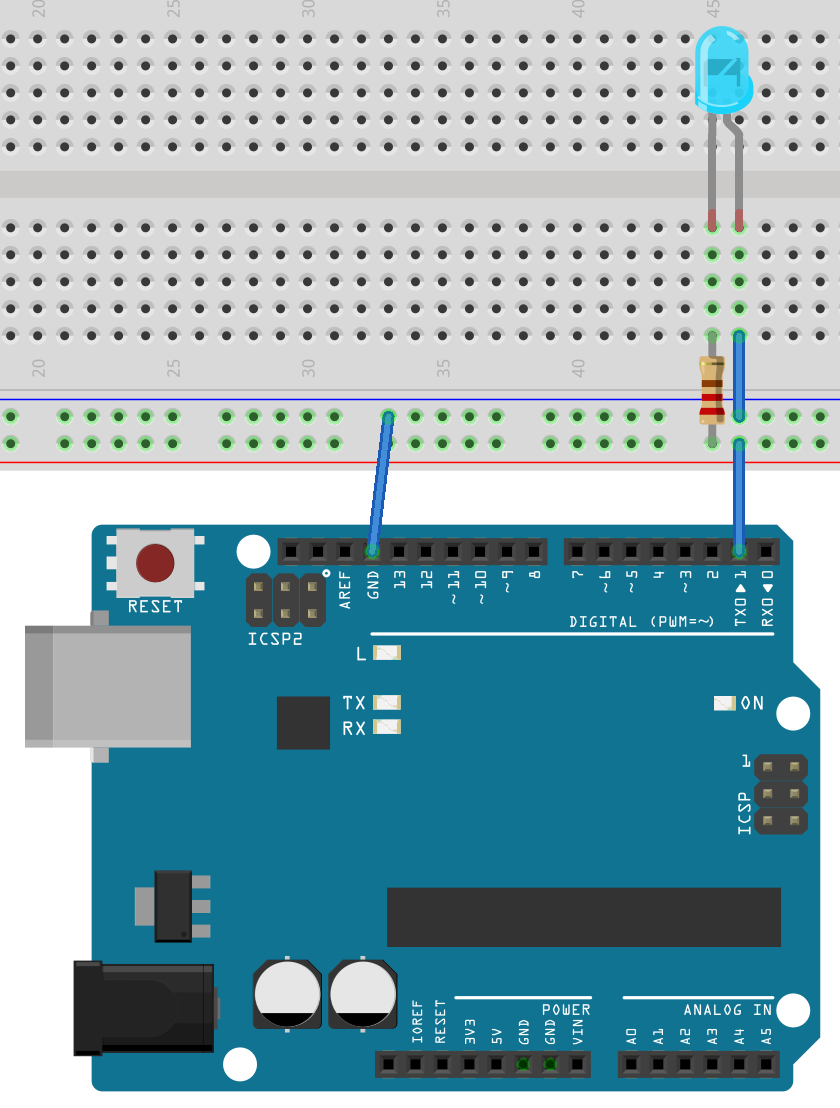
\includegraphics[width=\textwidth]{res/img/led}    
                \end{subfigure}
                \begin{subfigure}[b]{0.35\textwidth}
                    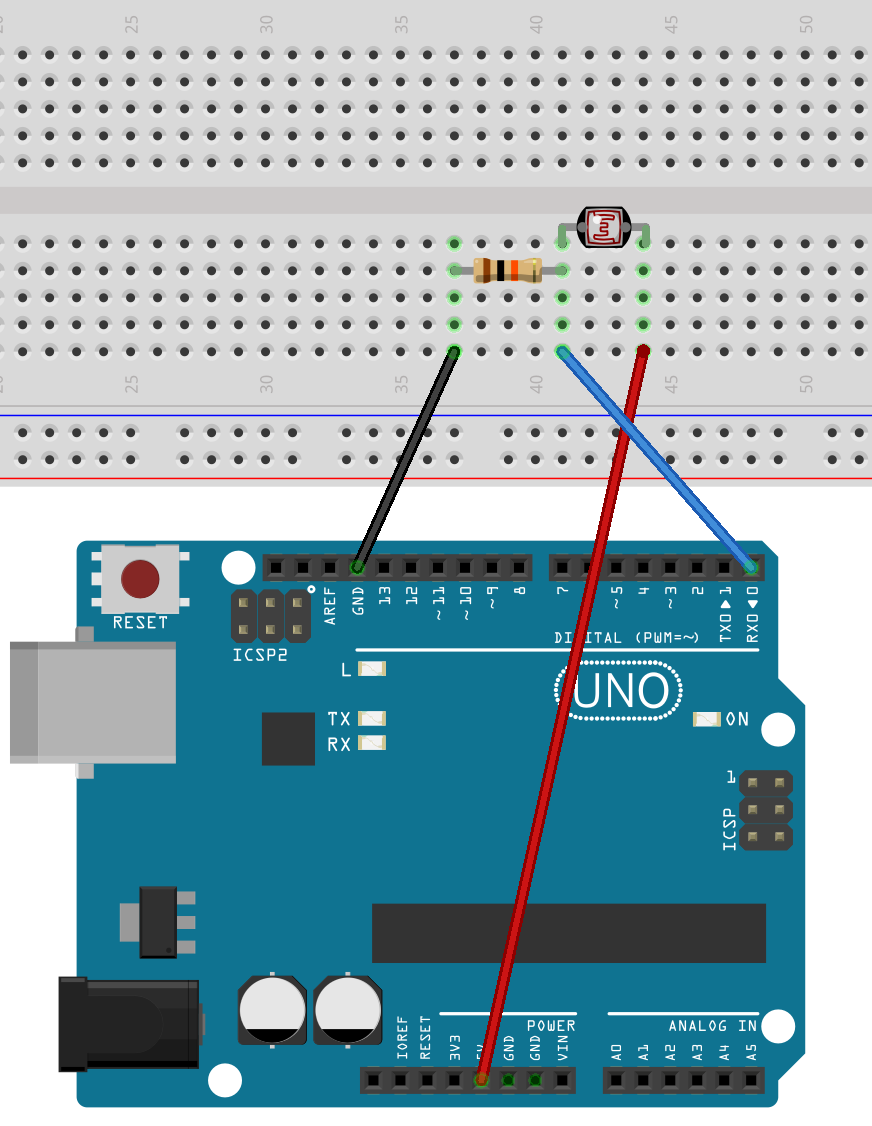
\includegraphics[width=\textwidth]{res/img/resistor}    
                \end{subfigure}
            \caption[Översikt av sändare/mottagare]{Översikt av sändare/mottagare. \\\tiny{Figuren skapad med hjälp av verktyget 'Fritzing'}}\label{fig:schema}
            \end{figure}

            För att möjliggöra överföringen användes den i förhållandevis låga överföringshastigheten om 300 baud, vilket gjorde att komponenterna (fotoresistorn och lysdioden) hann ändra sina värden under den tid de förväntades göra det. Komponenterna var inte särskilt utformade för denna uppgift och innehöll vissa fördröjningar vid skifte av tillstånd. \bigskip

            Den data som avsågs skickas i denna kommunikation bestod av ett 16 bitars värde, det vill säga två byte. Med en överföringshastighet om 300 baud ges en teoretisk möjlighet att skicka $\frac{300 \,\textit{baud}}{8 \, bit \cdot 2} = 18,75 \, \text{värden per sekund}$. Den faktiska hastigheten blir något lägre då extra bitar skickas enligt RS-232 protokollet, men överföringshastigheten var inte att anse som ett hinder i denna implementation. \bigskip
            
            Den andra lösningen använde sig endast av en luxmätare uppe på taket för att inhämta den data som efterfrågades. Genom att koppla samman två fibrer nere i rummet skickas ljuset åter upp till taket och en rundgång i systemet kan skapas. För att nyttja den här metoden behöver samtliga linser som tillhör en fiberkabel täckas över på panelen för att förhindra att dubbelt intag av solljus transporteras i de båda fiberkablarna. Kablarna är anpassade för att hantera den värme som produceras av det ljus som normalt transporteras vid fullt dagsljus men om den dubbla mängden skulle transporteras riskerar fibrerna att smälta på grund av värmebildningen. Lösningen använder sig inte av fiber som bärare av genererad information utan endast det solljus som panelen tar in skickas, vilket minskar både komplexiteten i systemet och risken för störningar.
        % subsubsection utformning_av_kommunikationslosning (end)

        \subsubsection{Utveckling av algoritm} % (fold)
        \label{ssub:utveckling_av_algoritm}
            Utformningen av algoritmen skedde genom flera iterationer av steg tre i den valda metoden. I den första iterationen utvecklades en sökalgoritm, algoritm $\mathscr{A}$, som genomförde medurs sökning i åtta riktningar med motsvarande österut som utgångsriktning. När ett större värde påträffats uppdateras nuvarande position och sökningen återupprepas. För jämförelse utvecklades även en variant med fyra sökriktningar, algoritm $\mathscr{B}$. Efterkommande iterationer var samtliga en vidareutveckling av den förra. Den andra iterationen gav algoritmen möjlighet att lagra information om tidigare besökta koordinater, så att dessa ej undersöks vid upprepade tillfällen. Ytterligare förbättringar implementerades i den tredje iterationen, då riktningen på den senaste förflyttningen registreras om ett nytt större värde påträffats. Med hjälp av denna information undersöks först samma riktning som den senast lyckade förflyttningen innan medurs sökning återupptas. Samtliga iterationer innebar märkbara förbättringar vid simulering. Efter tredje iterationen ansågs algoritmen vara funktionsduglig, den använder betydligt färre söksteg än tidigare versioner och hittar effektivt maximipunkten. Ett flödesschema över algoritmen finns i bilaga~\ref{sec:sokalgoritm_flow}.\bigskip

            \begin{figure}[b]
                \pgfplotsset{width=8cm,compat=1.8}
\begin{tikzpicture}
    \centering
    \begin{axis}[
        ybar,
        axis on top,
        % title={Söksteg algoritmer},
        height=5cm, width=10cm,
        bar width=0.3cm,
        ymajorgrids, tick align=inside,
        major grid style={draw=white},
        enlarge y limits={value=.1,upper},
        ymin=0, ymax=200,
        axis x line*=bottom,
        axis y line*=left,
        y axis line style={opacity=0},
        tickwidth=0pt,
        enlarge x limits=true,
        legend style={
            at={(0.5,-0.25)},
            % font=\footnotesize,
            anchor=north,
            legend columns=2,
            /tikz/every even column/.append style={column sep=0.5cm}
        },
        ylabel={Söksteg, median},
        symbolic x coords={version 1, version 2, version 3},
        xtick=data,
        % tick label style={font=\footnotesize},
        ]
        
        %% Median 8 riktningar
        \addplot [draw=none,fill=blue!60] coordinates {
            (version 1,215)
            (version 2,124) 
            (version 3,76)
        };

        %% Median 4 riktningar
        \addplot [draw=none, fill=red!60] coordinates {
            (version 1,140)
            (version 2,120) 
            (version 3,69)
        };
        \legend{$\mathscr{A}$: 8 riktningar,$\mathscr{B}$: 4 riktningar}
    \end{axis}
\end{tikzpicture}
            \caption{\label{fig:algoritm_steg} Jämförelse algoritmernas antal söksteg}
            \end{figure} 

            För att jämföra sökalgoritmerna genomfördes simuleringar som mäter antal steg från utgångspositionen till positionen där maximalt värde påträffas. Simuleringarna använde sig av 10\thinspace000 stycken 100$\times$100-matriser, där varje matris hade en slumpvis genererad utgångsposition och maximalt värde. Algoritmerna genomsökte identiska matriser med samma utgångsposition. Samtliga positioners värden var strängt avtagande med avseende på avståndet till det maximala värdet. För varje iteration av algoritmen undersöktes sökning med både fyra och åtta sökriktningar. Sökning i fyra riktningar visade sig mer effektivt i samtliga fall, enligt figur~\ref{fig:algoritm_steg} och bilaga~\ref{sec:sokalgoritm_sim}. Skillnaderna i antal steg mellan samma algoritm med olika antal sökriktningar vara störst i den första iterationen, med 54~\% fler steg, men de visade sig även i övriga iterationer. I den tredje och slutgiltiga iterationen var skillnaden 10~\% fler steg. Varje iteration av algoritmen minskade det antal steg som behövdes för att finna det största värdet. Största förändringen mellan iterationer skedde mellan iteration två och tre, där antalet steg minskades med 43~\%, se tabell~\ref{tab:algoritm_forbattring}. Minskningen mellan iteration ett och tre var 51~\%. \bigskip

            \begin{table}
                \caption{\label{tab:algoritm_forbattring}Minskning av antal söksteg mellan algoritmversioner}
                \centering
                \begin{threeparttable}
                \begin{tabular}{@{}lcc@{}}
                \toprule
                Från        & \multicolumn{1}{l}{Till version 2} & \multicolumn{1}{l}{Till version 3} \\ \midrule
                Version 1 & 14~\%                                & 51~\%                                \\
                Version 2 & -                                    & 43~\% \\ \bottomrule
                \end{tabular}
                \begin{tablenotes}
                \item Baserat på medianvärden, se bilaga~\ref{sec:sokalgoritm_sim}
            \end{tablenotes}
            \end{threeparttable}
            \end{table}


            % Trots att fokuspunkten inte är utformad på samma sätt som förutspått, fungerar sökalgoritmen så pass att den riktar in sig till det högsta funna värdet, dock på grund av panelens utformning av fokuspunkten finns det inget exakt högsta värde, utan algoritmen stannar i en punkt i den cirkel som panelen genererar. Algoritmen är inte utformad för att söka igenom hela cirkeln och sätta det högsta värdet, utan lokaliserar ett lokalt maximum. Detta ger ett högt belysningsvärde ut från panelen även om det kan finnas ett något högre värde existerar på motsatt sida av cirkeln. Skillnaden inom denna cirkel är dock så pass små att det rör sig om så små värdeskillnader att dessa kan anses ligga inom felmarginalen. Att utveckla en algoritm som arbetar sig igenom hela cirkeln är fullt möjlig, men det handlar om en avvägning om hur lång tid kalibreringen kommer ta, den nu gällande algoritmen är utvecklad för att hitta ett lokalt maximum på så få steg som möjligt.


        % subsubsection utveckling_av_algoritm (end)

        % \subsubsection{Utveckling av kommunikationslösning} % (fold)
        % \label{ssub:utveckling_av_kommunikationslosning}
        % % subsubsection utveckling_av_kommunikationslosning (end)

        \subsubsection{Avläsning av luxmätare} % (fold)
        \label{ssub:avlasning_av_luxmatare}
            De båda luxmätarna skiljer sig åt med avseende på det gränssnitt som förmedlar data. Mätaren från Adafruit kräver koppling till en mikrokontroller för tolkning av data, medan mätaren från Yoctopuce kopplas direkt till en enhet via USB, vilket underlättar anslutning till en persondator. Även om luxmätarnas gränssnitt skiljer sig åt beter sig de båda snarlikt vid användning. Båda generar ett positivt heltal som representerar uppmätt luxvärde och skickar detta när en metod i respektives bibliotek anropas. Från en programmerares perspektiv är resultatet från och användningen av de båda mätarna i praktiken identisk.\bigskip

            Vid kalibrering av panelen är det av intresse att inhämta så mycket av panelens ljus som möjligt när luxvärdet ska avläsas, samtidigt som bakgrundsljus från andra eventuella ljuskällor undviks, för att skapa mätbara skillnader mellan panelens olika kalibreringssteg. Luxmätaren placeras så nära fiberändan som möjligt för att säkerställa maximalt ljusintag från den panel som ska kalibreras, vilket i praktiken för detta projekt innebär tre till fyra centimeter från fibern. För att hålla mätaren stabil används olika metoder beroende på mätare, där den ena har monterats in i ett metallhölje som skruvas fast på fiberändan, medan den andra vilar i en armatur. Att metoderna skiljer sig åt beror på olika utformning av luxmätarnas mönsterkort och leder till att avlästa värden inte direkt kan jämföras.\bigskip 

            Testning av luxmätarnas inrapporterade värden visade att resultaten från solpanelen fluktuerar, vilket kan bero på orsaker så som att panelen ständigt justerar för att följa solen eller att något som momentant skuggar panelen passerar förbi. Dessa skiftningar i värde är inget som det mänskliga ögat uppfattar men blir synligt i mätningarna.\bigskip

            En undersökning av solpanelens solintag genomfördes i syfte att undersöka om panelens fokuspunkt överensstämmer med projektets antagande, figur~\ref{fig:array}. 
            Panelens justeringsvärden för ljussensorn stegades över ett kvadratiskt fält där ljusstyrkan avlästes och fördes in i en tvådimensionell matris.
            Resultatet av denna sökning gav olika bilder beroende på vilken luxmätare som användes. Den ena luxmätarens bild stämde inte överens med antagandet medan bilden från den andra stämde precis, vilket visas i figur~\ref{fig:luxcomp}.
            Hos Parans har tidigare efterforskningar aldrig resulterat i något liknande figur~\ref{fig:ada} och avvikelsen antas bero på luxmätaren Adafruit TSL2591. Att förlita sig till denna mätning skulle ge ett lägre ljusflöde från panelen då dess maximipunkt ligger i utkanten av äkta maximum.
            Projektet beslutade att endast använda den luxmätare som genererade förväntad fokuspunkt, Yoctopuce Yocto-Light-V3.
            Fullständig data från sökningen finns bifogad i bilaga~\ref{sec:heatmap}.

            \begin{figure}[h]
            \centering
                \begin{subfigure}{0.35\textwidth}
                    \setlength{\fboxsep}{0pt}
                    \fbox{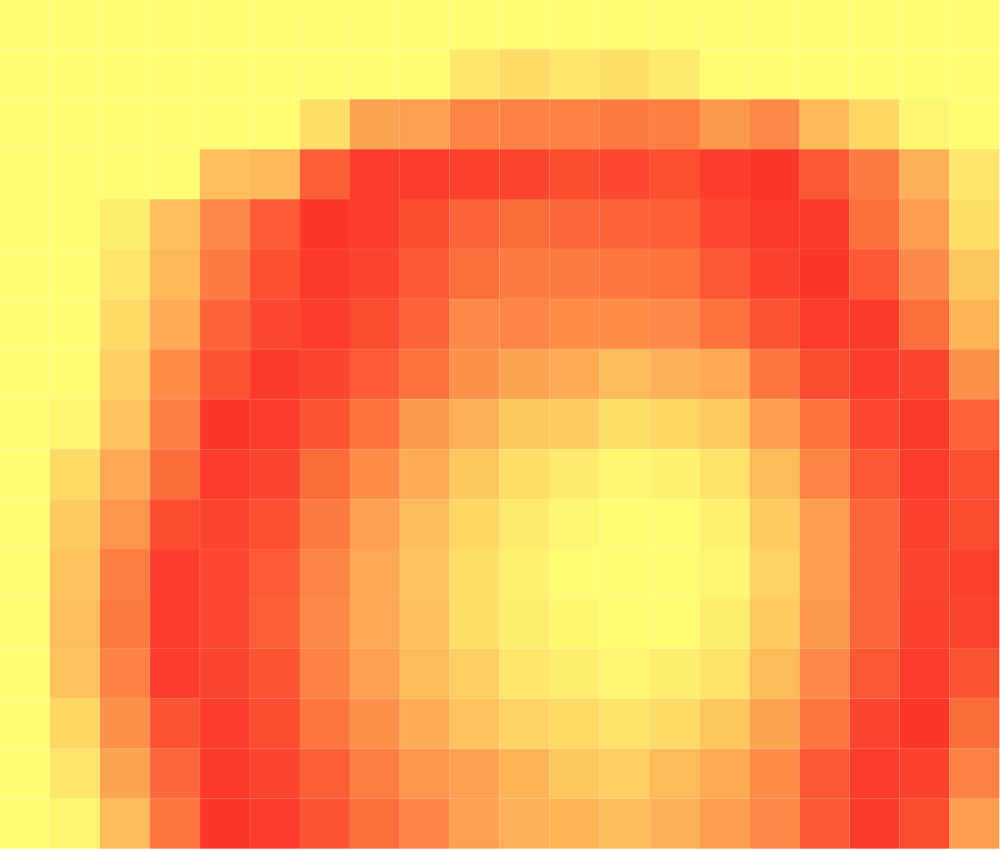
\includegraphics[width=\textwidth]{res/img/new_ada_23}}
                    \caption{\label{fig:ada}Luxmätare från Adafruit}
                \end{subfigure}
                \begin{subfigure}{0.35\textwidth}
                    \setlength{\fboxsep}{0pt}
                    \fbox{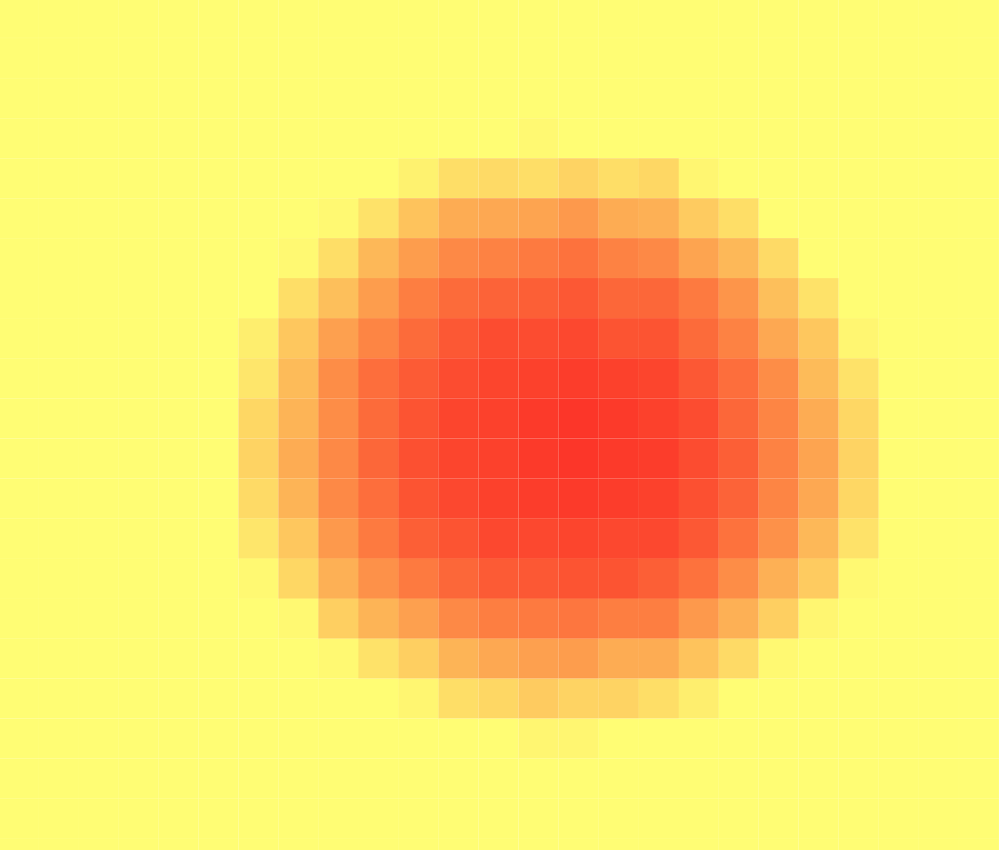
\includegraphics[width=\textwidth]{res/img/old_yocto_23}}
                    \caption{\label{fig:yocto}Luxmätare från Yoctopuce}
                \end{subfigure}
            \caption{\label{fig:luxcomp}Uppmätt ljusstyrka}
            \end{figure}
        % subsubsection avlasning_av_luxmatare (end)

        \subsubsection{Utveckling av applikation} % (fold)
        \label{ssub:utveckling_av_applikation}
            Efter att ha implementerat en algoritm som i simuleringar uppfyllde önskvärd funktion påbörjades utveckling av en applikation där den kan tillämpas. Förutom själva kalibreringsalgoritmen skulle applikationen ha egenskaper som kommunikation med panelen, ett användarvänligt grafiskt gränssnitt och inhämtning av värden från luxmätare. Programmeringsspråket som valdes för utveckling av applikationen var \texttt{Python} och valet hade stöd av flera motiveringar. Den första anledningen till att språket valdes var att företaget har kompetens och erfarenhet att utveckla i detta språk, då den nya panelen SP4 kommer att drivas av en källkod skriven i just \texttt{Python}. Att kompetens och kunskap finns inom företaget medför att applikationen kan underhållas av företaget själv och modifieras vid framtida behov. Vidare har företaget sedan tidigare produkter utvecklade i detta programmeringsspråk, så att utveckla applikationen i samma språk underlättar för en eventuell implementering av mjukvaran i de existerande produkterna. Mer generella fördelar med att utveckla i \texttt{Python} är att språket är plattformsoberoende och är enkelt att utveckla grafiska gränssnitt i. Nackdelar med språket är att det är långsamt i förhållande till andra språk såsom \texttt{C} eller \texttt{Java}. Då applikationen kommer att kommunicera med mekanik, vilket leder till flertalet fördröjningar för rotation av panelen och inhämtning och sändning av information, anser projektet att språkets åverkan på applikationens snabbhet är försumbar \cite{python_speed}. \bigskip

            För att kommunicera med panelen och den Arduino som mottar värden från luxmätaren Adafruit TSL2591 behövdes stöd för seriell kommunikation. Ett bibliotek som möjliggjorde seriell kommunikation med enheter anslutna till en dator var pySerial. Eftersom pySerial har stöd för operativsystem baserade på Windows, Linux och BSD är biblioteket i praktiken plattformsoberoende \cite{pyserial}. \bigskip

            Till luxmätaren Yocto-Light-V3, som anslöts direkt till den dator som kör applikationen, fanns kodbibliotek för \texttt{Python} att tillgå från tillverkaren Yoctopuce. \bigskip

            Till det grafiska gränssnittet fanns flera tillgängliga ramverk som var utvecklade och anpassade till \texttt{Python}. Det som ansågs mest lämpligt för applikation var TkInter, där en anledning är att Parans sedan tidigare har kringutrustning som använder TkInter \cite{solarremote}. Hänsyn togs till att underlätta både framtida hantering av koden för bolaget och en eventuell integrering av tidigare produkter med den av projektet utvecklade applikationen. En annan anledning är att ramverket distribueras med standardinstallationer av \texttt{Python} till Windows och Mac OS X \cite{tkinter}. På Linuxsystem behövs TkInter installeras separat och det finns tillgängligt i flera stora Linuxdistributioners pakethanterare. Behovet av extra installationer för ett ramverk kunde minimeras och det grafiska gränssnittet kunde göras plattformsoberoende. \bigskip

            För att underlätta framtida hantering av den producerade koden eftersträvades en modulär uppbyggnad av applikationen. Inledningsvis isolerades den framtagna algoritmen i en egen klass, \texttt{Search}. Anslutningarna till panelen och de olika luxmätarna implementerades i separata klasser med specifik kod för att hantera varje enskild enhet. För att hantera de olika anslutningarna skapades klassen \texttt{SerialHandler} som ett mellanliggande gränssnitt till applikationens övriga komponenter. För att kompensera för de fluktuerande värden som beskrevs i avsnitt~\ref{ssub:avlasning_av_luxmatare} hämtar \texttt{SerialHandler} fyra luxvärden från en ansluten mätare och medelvärdet av de två mellersta rapporteras vidare för att få en bättre uppskattning vid kalibreringen. Det grafiska gränssnittet hanteras av klassen \texttt{GUI} och där skapades tryckknappar för att aktivera applikationens funktioner och ett fält för återkoppling och presentation av information. De tre klasserna \texttt{Search}, \texttt{SerialHandler} och \texttt{GUI} fick tillsammans utgöra grundstommen i applikationen och utformades för att vara plattformsoberoende. Genom att sökalgoritmen och det grafiska gränssnittet endast använder sig av det mellanliggande gränssnittet i \texttt{SerialHandler} och ej de underliggande anslutningarna uppnåddes en mer modulär design och ett oberoende av de implementationsspecifika delarna av applikationen. En översikt av klasserna finns i bilaga~\ref{sec:uml_diagram}. \bigskip

            Då applikationen är beroende av anslutning till externa enheter lades funktionalitet till för att underlätta anslutningen. Applikationen kan användas på olika plattformar och olika förfaranden framställdes för olika operativsystem. Stöd för automatisk identifiering av ansluten panel och Arduino implementerades till Mac OS X och Linux. Förutsättningen för detta var att inga fler externa enheter av samma typ är anslutna till den aktuella datorn. För Windowssystem utvecklades en dialogruta som vid applikationsstart frågar användaren efter de aktuella COM-portarna för respektive enhet. Om ingen Arduino är tillkopplad försöker applikationen använda sig av Yocto-Lux-V3. \bigskip

            Det grafiska gränssnittet gavs en enkel design och baserades på det utseende som används i företagets kringutrustning \cite{solarremote}. Nämnda kringutrustning var utformad för att kunna användas med pekskärm och således beaktades detta även här. Fyra knappar i form av ett styrkors lades till för att manuellt ändra panelens justeringsvärden för ljussensorn i x- och y-led. I mitten av styrkorset placerades en knapp för manuell avläsning av den anslutna luxmätaren. Nedanför styrkorset placerades en knapp som startar automatisk kalibrering och en knapp som återställer panelens justeringsvärden till de som var aktuella vid applikationens starttillfälle. Ett fält som kan förmedla aktuell information placerades i applikationens underkant. Det grafiska gränssnittet är avbildat i figur~\ref{fig:app_skiss}.

            \begin{figure}[hb]
                %%% Illustration of the application used for calibration %%%

\begin{tikzpicture}[font=\sffamily\footnotesize]
    % Outer rectangle
    \draw (0,0) rectangle (6,8);

    % Top line
    \draw (0,7.5) -- (6,7.5);

    % Bottom line
    \draw (0,0.8) -- (6,0.8);

    % Window functions
    \draw (5.85,7.85) -- (5.65,7.65);           % Close diagonal 1
    \draw (5.85,7.65) -- (5.65,7.85);           % Close diagonal 2
    \draw (5.26,7.67) rectangle (5.42,7.83);    % Maximize (square)
    \draw (4.84,7.75) -- (5.00,7.75);           % Minimize (line)
    \draw (0.2,7.61) rectangle (0.45,7.87);     % Left square
    \draw (0.2,7.84) rectangle (0.45,7.84);     % Line on left square

    % Buttons
    \draw (2.2,7.3) rectangle (3.7,5.8);    % Up
    \draw (0.5,5.6) rectangle (2.0,4.1);    % Left
    \draw (2.2,5.6) rectangle (3.7,4.1);    % Middle
    \draw (3.9,5.6) rectangle (5.4,4.1);    % Right
    \draw (2.2,3.9) rectangle (3.7,2.4);    % Down
    \draw (0.2,1.0) rectangle (2.0,1.7);    % Left corner
    \draw (5.8,1.0) rectangle (3.9,1.7);    % Right corner

    % Text
    \draw (2.2,7.73) node {Panel calibration};
    \draw (2.95,6.55) node {UP};
    \draw (1.25,4.85) node {LEFT};
    \draw (2.95,4.85) node {VALUE};
    \draw (4.65,4.85) node {RIGHT};
    \draw (2.95,3.15) node {DOWN};
    \draw (1.1,1.35) node {SEARCH};
    \draw (4.85,1.35) node {RESET};
    \draw (2.9,0.55) node {Information box};
    \draw (3.0,0.20) node {Application status is presented here};
\end{tikzpicture}

            \caption{\label{fig:app_skiss} Skiss av det grafiska gränssnittet}
            \end{figure}

        % subsubsection utveckling_av_applikation (end)

    % subsection steg_3 (end)

    \subsection{Fas 4} % (fold)
    \label{sub:fas_4}
        Den fjärde fasen i den valda metoden avhandlar inte arbetsgången som sådan, utan visar på att resultatet från den tredje fasen ska analyseras och delges i syfte att sprida kunskapen om vad som har uppnåtts vidare. 
        För detta projekt innebar fas fyra att skriva denna rapport vilket förtydligar och sammanfattar det resultat som har uppnåtts genom de iterationer som genomförts. Vidare hålls en presentation av resultatet inom ramen för den kurs som genomförs, vilket även är en del av metoden.
    % subsection fas_4 (end)
% section genomf_rande (end)
\section{Resultat} % (fold)
\label{sec:resultat}
    \subsection{Algoritm} % (fold)
    \label{sub:algoritm}
        För att möjliggöra automatisk kalibrering av panelens ljussensor har projektet utvecklat en sökalgoritm med positionsregistrering och stegreducering. Den utvecklade algoritmen gav svar på den första av projektets tre frågeställningar, ''Vilken algoritm kan anses vara lämplig för kalibreringen?''. Algoritmen uppsöker ett lokalt maximum i ljusstyrka, beskrivet i avsnitt~\ref{ssub:utveckling_av_algoritm}, och fanns lämplig för ändamålet.\bigskip

        Algoritmen söker stegvis efter det maximala inlästa värdet tills inga kringliggande större värden påträffas. I varje söksteg justeras panelens korrigeringsvärde för ljussensorn, vilket får panelen att vrida sig till den position som ger solljusets fokus i ljussensors korrigerade mittpunkt. Sökning sker i fyra riktningar, representerade av väderstrecksuttryck motsvarande den koordinatsystemsrepresentation panelen har för korrigeringsvärden där positiva x och y är öst respektive nord, och sker medurs med utgångsriktning österut. Om ett lika stort eller större värde avläses efter en vridning av panelen så kommer nästkommande undersökta position vara i samma riktning som den senast utförda, då avlästa värden antas vara kontinuerligt fallande från maximipunkten. Detta i enlighet med initialt antagande, representerat i figur~\ref{fig:array}, och senare undersökning, enligt figur~\ref{fig:yocto}. Algoritmen registrerar besökta positioner så att samma position ej undersöks upprepade gånger. Flödesschema för algoritmen finnes i bilaga \ref{sec:sokalgoritm_flow}. \bigskip

        Tillgången till kontinuerligt solljus är en förutsättning för kalibrering av enheter tagna i bruk då variationer i molnighet markant påverkar ljusintensiteten och således det avlästa värdet. I händelse av längre tids molnighet deaktiveras ljussensorn av panelens mjukvara och kalibrering går då ej att genomföra. Om så sker under pågående kalibrering återställs panelens korrigeringsvärden till de värden som var aktuella innan den automatiska kalibreringen startade. För att ytterligare motverka oförutsedda problem vid kalibreringstillfället har kontroller för timeout och korrigeringsvärdenas rimlighet implementerats, där båda kontrollerna vid utslag avbryter sökningen och korrigeringsvärdena återställs.

    % subsection algoritm (end)
    \subsection{Optisk kommunikation} % (fold)
    \label{sub:optisk_kommunikation}
        För att svara upp mot målet att ta fram en lösning för ''kommunikation mellan en luxmätare inne i byggnaden och en panel som befinner sig på taket'' besvaras i efterföljande frågeställningar för förutsättningar för kommunikation och hur tillförlitliga dessa lösningar kan anses vara.

        \subsubsection{Förutsättningar} % (fold)
        \label{sub:forutsattningar}
                
            Frågeställningen ''[v]ilka förutsättningar för kommunikation finns det mellan solpanelen och det upplysta rummet'' har resulterat i en undersökning som visade att trådlös kommunikation inte är att anse som lämplig, utan den redan dragna optiska fiberkabeln är det kommunikationsmedia som bör nyttjas. Projektet föreslår två olika metoder för att nyttja fibern som databärare, dels en metod där asynkron seriell data skickas och en annan metod där två optiska fibrer kopplas samman, för att på sådant sätt skicka ut ljusintaget genom panelens linser och där uppmäta ljusstyrkan.\bigskip

            Den första lösningen som projektet föreslog var att en mikrokontroller inne i det upplysta rummet omvandlar utdata från en luxmätare till en optisk signal som sedan sänds seriellt, enligt standarden RS-232, upp till panelen för att där avkodas av en andra mottagande mikrokontroller. När signalerna skickas via fibrerna strålas ljuset ut ur solpanelens linser, vilket mottagaren då kan analysera. Mottagaren är monterad på panelen och har en ljuskänslig sensor som omvandlar de optiska signalerna till digitala. De digitala signalerna skickas från mottagaren vidare till den enhet som utför den algoritm som är avsedd att kalibrera ljussensorn. \bigskip

            Den andra lösningen var att, istället för att mäta upp ljusstyrkan i rummet, koppla ihop två stycken optiska fibrer från samma panel i det rum de är avsedda att upplysa, vilket då skickar ljusintaget tillbaka upp till panelen. Genom att täcka över de linser som förser den ena fiberkabeln med ljus kommer den andra fiberkabeln att skicka ut sitt ljusintag mot de nu täckta linserna. I detta förslag kan en luxmätare placeras i övertäckningsanordningen och där, via omvägen till det upplysta rummet och tillbaka, mäta upp hur mycket ljus panelen tar emot. Då luxmätaren nu befinner sig på panelen kan den direkt skicka sin data till den enhet som förväntas utföra algoritmen.

        % subsection förutsättningar (end)

        \subsubsection{Tillförlitlighet} % (fold)
        \label{sub:tillf_rlitlighet}
            För att komma fram till ett svar på frågan ''[h]ur tillförlitligt är det valda kommunikationssättet?'' utreddes flera alternativ för att sända data. Genom att använda de fördragna fiberoptiska kablarna säkerställs att det ljus som skickas från rummet upp till panelen alltid kommer att levereras, förutsatt att ljuskällan är tillräckligt stark. Detta är i skarp kontrast mot en trådlös lösning, där flera lager betong mellan rummet och panelen inte är en osannolik företeelse vilket då skulle resultera att datan aldrig når till panelen under normala förutsättningar. \bigskip

            Huruvida de två föreslagna lösningarna för ljussändning är tillförlitliga är beroende på hur ljuset läses av uppe vid panelen. I förslaget med två mikrokontroller, där data sänds seriellt via RS-232, är tillförlitligheten lägre, då den lösningen är störningskänslig mot bakgrundsljus så en tillförlitlig fästningsanordning för panelen behöver tillverkas. Vid försök i labbmiljö har data kunnat sändas med hjälp en vanlig lysdiod driven av 5 volt, 20 mA via en fiberkabel om 16 meter och där tolkats från en enskild fiber. Varje fiberkabel består av sex stycken fibrer och varje fiber är kopplad till en egen lins för att fokusera in soljuset. Nu när data skickas nedifrån och upp kommer linsen att agera omvänt genom att omvandla fiberns fokuserade ljus till parallella strålar. Då ljuset nu är parallellt istället för fokuserat finns det risk att ljusintensiteten mellan hög och låg inte är tillräckligt stor för att fotosensorn ska registrera skillnaden, eller ändra sitt motstånd tillräckligt mycket. För att fotoresistorn ska ha möjlighet att registrera ljusändringarna hade det ideala varit en fokuseringslins till fotoresistorn och att resistorn hade varit innesluten i någon form av behållare att fästa över de sex linserna. \bigskip

            Det andra förslaget, där två fiberkablar kopplas samman för att skapa rundgång, är tillförlitligheten högre eftersom ingen behandlad data skickas. Ingen kommunikation behöver läsas av utan endast rådata i form av ljusstyrka skickas ut genom linserna. När ljusstyrkan då ska mätas är luxmätaren inte beroende av snabba ändringar i ljuset, utan ljuset är konstant vilket leder till en högre tillförlitlighet. Ljusstyrkan kommer vara lägre när den kommer upp till panelen, jämfört med om den skulle stråla ut i rummet, då den behöver färdas dubbelt så långt i fiberkabeln, men mätningen av ljusstyrkan är inte beroende av ett korrekt absolut värde. När panelen kalibreras är det istället av intresse att finna det högsta relativa värdet, det värde när panelen tar in mest ljus, för det är ljust där som panelen ska vara inställd på, oavsett vilket värde som projektets luxmätaren nu rapporterar. Detta medför också att denna metod är mindre känslig för bakgrundsljus, så länge bakgrundsljuset är konstant eftersom skillnaden i det utstrålade ljuset ändå kan registreras.\bigskip 

            För att kontrollera vilket luxvärde panelen faktiskt levererar till rummet behövs mer kvalificerad utrustning användas, som är kalibrerad och granskad för att mäta luxvärden i rum. Det är apparatur som företaget har tillgängligt men som ligger utanför detta projekt.
        % subsection tillf_rlitlighet (end)
    % subsection optisk_kommunikation (end)

    \subsection{Applikation} % (fold)
    \label{sub:applikation}
        Den framtagna applikationen gav en förutsättning att uppfylla målet ''att ta fram ett automatiskt system som justerar fokuspunkten på ljussensorn''. En automatisk kalibrering av panelens korrigeringsvärde för ljussensorn kan utföras genom att applikationen har kopplat samman sökalgoritmen med solpanelen och en luxmätare.\bigskip

        Sökalgoritmen implementerades i form av en Pythonapplikation med grafiskt gränssnitt och applikationen stödjer inhämtning av ljusvärden från antingen en till samma dator direkt ansluten luxmätare eller seriell mottagning från en annan enhet. Den luxmätare som användes vid implementationen av direkt anslutning var Yocto-Light-V3 medan Adafruit TSL2591 användes för avläsning som sedan överfördes seriellt via en Arduino Uno. Luxmätarna är beskrivna i avsnitt \ref{sub:yocto} respektive \ref{ssub:ada_tsl2591}. För seriell kommunikation använder applikationen sig av pySerial, ett bibliotek som kan hantera seriell kommunikation på de flesta vanligt förekommande operativsystem \cite{pyserial}. \bigskip

        Hos Parans fanns sedan tidigare kringutrustning som använder en Pythonapplikation med grafiskt gränssnitt anpassat till en pekskärm på en Raspberry Pi, där det grafiska gränssnittet är implementerat med ramverket TkInter \cite{solarremote}. Samma ramverk och grafiska formgivning har använts till den applikation som utvecklats av projektet. Detta upplägg är tänkt att underlätta framtida hantering och utveckling av applikationerna och möjliggör en eventuell framtida integrering av de båda. \bigskip

        Applikationen är utvecklad enligt en objektorienterad utvecklingsmodell och nya avläsningsmetoder kan implementeras utan större ingrepp i befintlig kod. För en översikt av källkodens struktur se UML diagrammen i bilaga~\ref{sec:uml_diagram}. Mjukvaran till Parans kommande solpanel, SP4, var ej färdigställd under projektets gång och således är applikationen riktad till SP3. Implementeringen av sökalgoritmen kan återanvändas till kommande versioner av solpaneler men vissa anpassningar kan behövas.
    % subsection applikation % (end)
% section resultat (end)

\section{Diskussion} % (fold)
\label{sec:diskussion}

    Projektet är kan anses ha två huvudsakliga syften, där det första syftet är att ''ta fram en helt automatisk process som kan kalibrera fotosensorn i Parans solpaneler [~\dots~] med en lägre tidsåtgång och högre precision än dagens manuella metod''. 
    Den metod som företaget använde sig av tidigare, var dels baserad på manuell inmatning av värden, vilket tar tid och kan leda till fel på grund av den mänskliga faktorn och dels en manuell uppskattning av ljusstyrkan vilket även det kan leda till en felaktig kalibrering. 
    Med hjälp av den algoritm som projektet har utvecklat och redovisat, anser författarna att detta syfte är uppnått. Processen kan skötas helt automatiskt, så till vida att ljusflödet ut från panelen kan uppmätas. 
    Denna automatiserade kalibrering är att anses som tidsparande då inga värden behöver anges manuellt vilket sparar tid, särskilt då skillnaden mellan sensorns optimala inställningsvärde och det ursprungliga värdet är stort, så att många kalibrerings steg behöver göras. \bigskip

    Gällande bestämningen av ljusintensiteten finns det både för- och nackdelar mellan att göra en uppmätning av ljusstyrkan och en mänsklig uppskattning. Fördelarna med en automatiserad inläsning av ljusstyrkan är att kalibreringen blir standardiserad och inte behöver bero på personen som utför kalibreringen. När författarna deltog i ett praktiskt exempel av kalibrering av panelen ute i produktion upplevde vi att ljusintensiteten varierar väldigt mycket och med tanke på det mänskliga ögat och att dess anpassning till olika ljusintensiteter varierar olika snabbt beroende på om ljusintensiteten ökar eller minskar, kan kalibreringen tappa i precision vid en manuell bedömning.\cite[s.~273]{aot}  Det är svårt att jämföra hur två inställningar förhåller sig till varandra, vilken som är starkare eller svagare, om ljuskällan blivit väldigt mörk mellan de båda tillfällena. Det ska dock påpekas att en rent mekanisk bedömning har sina brister då ''[d]et är i det närmaste omöjligt att planera ljusmiljö [ \dots ] enbart med hjälp av fysikaliska mätningar'' men det påpekas också i litteraturen att det krävs erfarenhet för att kunna göra lämpliga bedömningar. \cite[s.~278]{aot} Personer med den erfarenheten finns sällan att tillgå för företaget då deras tekniker inte har möjlighet att befinna sig i rummet dit ljuset leder, utan befinner sig vid panelen för att sköta kalibreringen. Sammantaget är vår bedömning att en uppmätning av ljusstyrkan är den mest lämpliga metoden då det sparar tid vid kalibreringen och blir oberoende på operatörers erfarenhet gällande bedömning av ljusintensitet.

% section diskussion (end)

\newpage
\printbibliography
\addcontentsline{toc}{section}{Referenser}

\newpage

\setcounter{page}{1}
\pagenumbering{Roman}
\appendix

\end{document}